\begin{savequote}[45mm]
  When you plant a fertile meme in my mind you literally parasitize my brain,\
  turning it into a vehicle for the meme's propagation in just the way that a\
  virus may parasitize the genetic mechanism of a host cell.
  \qauthor{Richard Dawkins \cite{dawkins2006}}
\end{savequote}

\chapter{Introducción}

\noindent
El siglo XXI ha traído consigo una transformación radical en las formas de comunicación\
entre personas. Hoy en día, el uso de redes sociales \emph{democratiza} el acceso\
a la información más relevante ocurriendo en tiempo real, sin tener que esperar a que un medio\
masivo publique una noticia sobre ello. Cualquier persona con una cuenta de \textit{Twitter}\
\footnote{Red social de intercambio de mensajes cortos. URL: \url{http://www.twitter.com}} puede\
tomar una fotografía, subirla a la \textit{web} y etiquetarla de la manera en que más le convenga (mediante\
\textit{hashtags}, por ejemplo). Dependiendo de muchos factores, incluyendo el alcance del\
\textit{tuit} y el número de seguidores de la cuenta de Twitter, es posible que la imagen se vuelva\
más popular de lo que una nota publicada por algún periodista serio pueda alcanzar.\par
Este fenómeno también se explica por las intenciones que llevan a la gente a interactuar dentro de\
las redes sociales. Al usuario se le da la libertad de hacer que el contenido de su \textit{timeline (TL)}\
sea tan ocioso, o tan serio, como éste quiera, siguiendo en el caso de Twitter. Cuando un tuit acompañado\
de una imagen se vuelve \emph{viral}, surge un fenómeno de propagación en el cual el poder del\
\textit{tuitero} permite re-etiquetar la imagen sin perder la esencia de la idea original transmitida\
por la misma.\par
En general, este fenómeno no es exclusivo de Twitter y ha ocurrido en Internet desde que la comunicación\
entre personas se efectuaba exclusivamente por medio de correos electrónicos. Para englobar a las diversas\
maneras en las que se ``viraliza'' cierta información en la web en un solo concepto, se ha popularizado el\
término \emph{\textbf{meme (de Internet)}}, el cual pretende \emph{discretizar} la información cultural\
en unidades capaces de pasar de persona a persona, gradualmente escalar en un fenómeno social compartido\
e incluso \emph{evolucionar} \cite{shifman2014}.\par
Paralelamente, el constante incremento en el uso de redes sociales genera un cúmulo de datos esparcidos\
por el Internet. De acuerdo al un estudio descrito en \cite{website:smartinsights} y publicado en 2016,\
el $46\%$ de la población mundial son usuarios de Internet y el $31\%$ son usuarios activos de alguna red social.\
Además, durante 2015 se produjo un aumento de usuarios equivalente a $10\%$ en los dos rubros descritos anteriormente.\
Consecuencia de esto es que a diario, el intercambio de información favorece a la riqueza y complejidad\
de nuevas ideas que se acumulan en grandes servidores pero cuya relevancia está empezando a ser explorada.\par
Dentro de la rama de las ciencias de la computación, conocida como \textbf{inteligencia artificial}, el\
\textbf{aprendizaje automático} (\emph{machine learning} en inglés) propone técnicas capaces de lograr que, a partir\
de grandes cantidades de datos, un sistema de cómputo revele información oculta para muchos seres humanos.\
El auge del subconjunto de \emph{algoritmos de aprendizaje} automático conocido como\
\textbf{aprendizaje profundo} (\emph{deep learning} en inglés), trae consigo un importante adelanto\
en el desempeño de computadoras al realizar habilidades humanas. Dos ejemplos significativos incluye el reconocimiento\
de imágenes y rostros mediante visión computacional y la generación automática de texto coherente en algún idioma.\par
Motivado por lo establecido en los párrafos anteriores, en el presente trabajo se explorarán dos modelos de\
aprendizaje profundo para entrenar, identificar y, finalmente, etiquetar memes de Internet. Se considerará únicamente\
el caso de una imagen (la cual, en el la mayoría de los casos, incluye a un solo personaje) y una \emph{leyenda} asociada.\
Por lo tanto, se presentará un método para hacer que la computadora aprenda al personaje dentro del meme y la información\
textual que transmite; posteriormente se experimentará etiquetando memes no antes vistos por dicha computadora.

\section{Memes de Internet y \emph{memética}}

\noindent
El término \emph{meme} fue acuñado por el biólogo Richard Dawkins en su libro \emph{``The Selfish Gene''}\
de 1976. Mediante una analogía con el papel del \emph{gen} en la evolución darwiniana, Dawkins\
propuso una teoría cultural en la cual el meme es visto como la unidad que se propaga por generaciones\
y sobrevive mediante un proceso semejante a la selección natural. Dawkins conjeturó que la teoría de la evolución\
de Darwin es una instancia particular de un proceso que se puede encontrar en otras áreas; en particular,\
es suficiente que cualquier concepto que incorpore las propiedades de \emph{longevidad}, \emph{fecundidad} y\
\emph{fidelidad de copias} para que éste tenga un comportamiento evolutivo a través del tiempo \cite{distin2005}.\par
Hoy en día, se le conoce como \emph{meme} principalmente al objeto proveniente de Internet y que incorpora,\
en el mayor de los casos, una imagen y una leyenda que cuenta algo sobre la imagen. Es importante recalcar\
el aspecto humorístico, muchas veces incluso irónico, que caracteriza al meme de la actualidad ya que ello\
contribuye a la difusión de los mismos por la web. Sin embargo, es el diseño \emph{centrado al usuario} característico\
de la llamada \emph{Web 2.0} lo que mayormente facilita la propagación de memes.\par
Dentro de esta estructura tecnológica, las tres propiedades adscritas por Dawkins a cualquier objeto evolutivo se\
satisfacen para los memes: la digitalización permite una transmisión casi sin interferencias (fidelidad de copias),\
el número de copias compartidas en una unidad de tiempo es gradual -- dada la facilidad de compartir información\
``de nodo a nodo'' -- (fecundidad) y el aumento en la longevidad de la información es respaldado por la capacidad de\
almacenamiento indefinido en los servidores de la web. \emph{Reddit}\
\footnote{Sitio web de marcadores sociales e intercambio de enlaces a contenidos de Internet. URL: \url{http://www.reddit.com}}\
es uno de los sitios web con mayor flujo y contenido de memes; su eslogan \emph{``the front page of the Internet''}\
resume la importancia cultural que el alcance de su contenido modifica las formas de obtener y discutir información\
de cualquier índole. Lo que Dawkins no se imaginó en los años 70's es que el meme se convertiría en la mejor\
manera de encapsular los aspectos más fundamentales de Internet \cite{shifman2014}.

\begin{figure}
  \centering
  
\includegraphics[width=0.5\textwidth]{success_kid}
  \caption{Clásico ejemplo de un personaje \emph{memificado} junto con una de sus
    leyendas (descripciones). (Tomado de \url{http://www.memegenerator.net}.)}
\end{figure}

La trascendencia del concepto de Dawkins provocó el surgimiento de la \emph{memética}, la disciplina\
sociobiológica que extrapola el concepto de evolución de la teoría de Darwin para colocar al\
meme como instrumento de supervivencia, un \emph{replicador}. Originalmente, Dawkins sugirió como\
ejemplos de memes a frases pegadizas, tonos de audio, modas, habilidades o simplemente ideas.\
Más aún, según Dawkins el meme es una ``unidad de información que reside en un cerebro'' \cite{dawkins2006},\
una afirmación que sugiere la relevancia que el alcance de las redes sociales tiene en la población\
actual, incluso mayor a la que otros medios de comunicación -- como la televisión o la radio -- alcanzaron\
desde su concepción.

\section{Un esbozo sobre el aprendizaje profundo}

\noindent
El ser humano es complejo. Desde una perspectiva computacional, cualquier persona realiza tareas que constituyen\
una inteligencia que hasta más de la mitad del siglo XX parecía inimitable. Por otro lado, si hay\
una capacidad para la cual el cómputo actual ha superado a la inteligencia humana es la de procesar números;\
la computadora es, abstractamente, una máquina que entiende muy bien cadenas de ceros y unos. La apuesta moderna\
consiste, entonces, en transformar las habilidades humanas en problemas numéricos para los cuales la computadora\
puede \emph{aproximar} una solución.\par
Una de las primeras maneras de estudiar a la inteligencia humana, de manera computacional, pretende resaltar las\
capacidades de buscar y encontrar caminos para resolver situaciones complicadas (en juegos, por ejemplo). Al\
implementar algoritmos de búsqueda de soluciones, es inminente encontrarse de frente con casos en los que las\
capacidades de una computadora, por más nueva y equipada que sea, no sea suficiente para lograr un desempeño\
equiparable al del ser humano. En términos más formales, se dice que el tamaño del \emph{espacio de estados},\
el cual define el conjunto de conocimiento que puede tener un \emph{agente racional} mientras llega a una meta,\
se vuelve computacionalmente intratable. Las técnicas más innovadoras, en inteligencia artificial, para\
tratar con problemas corresponden a la modelación del entorno de un agente de manera numérica y a la aproximación\
de resultados por medio de algoritmos probabilísticamente efectivos \cite{russell2010}.\par
Si a lo establecido anteriormente se le suma la tendencia a elaborar modelos\
matemáticos que \emph{``aprenden''} mediante una gran cantidad de ejemplos, encontramos a lo que se conoce como\
\emph{aprendizaje automático}. Estadísticamente hablando, aprender significa que estos modelos \emph{convergen} a\
un estado deseado dependiendo de la tarea a realizar. Cuando la robustez del algoritmo (o \emph{heurística}) numérico\
propuesto depende directamente de la existencia de un conjunto de datos de \emph{entrenamiento}, se habla de\
un \textbf{aprendizaje supervisado}. En ausencia un conjuntos de datos, es posible realizar búsquedas\
de patrones sobre datos desconocidos; a esto se le conoce como \textbf{aprendizaje no supervisado}.\par
El cerebro humano no es solamente una máquina que pueda procesar información. En este sentido, la inteligencia\
artificial se ha inspirado en la anatomía del sistema nervioso para perfeccionar al aprendizaje automático.\
Con esto surgen los modelos conocidos como \textbf{redes neuronales}: arquitecturas de neuronas interconectadas\
que, dado un conjunto de ejemplos, buscan fortalecer ciertas conexiones para construir un modelo abstracto sobre\
la realidad observada por un agente (en el caso \emph{supervisado}). Los conceptos introducidos en estos dos últimos\
párrafos serán profundizados en el siguiente capítulo.\par
El modelo más simple de una red neuronal corresponde al del perceptrón, el cual puede ser visualizado como un conjunto\
de neuronas que reciben la información (\emph{de entrada}) y que se combinan en una neurona \emph{de salida}.\
Posteriormente, apilando varios perceptrones en \emph{capas}, se logran modelos más complejos. Dependiendo de la\
conexidad de cada capa, de la dirección hacia donde fluye la información y de la existencia de ciclos en el modelo,\
surge una especie de \emph{``zoológico de redes neuronales''} (término acuñado en \cite{website:theasimovinstitute}).\
El éxito en la consecución de estos modelos consiste en el incremento en el número de capas de\
neuronas. Cuando un modelo alcanza una cantidad cosiderable de las mismas, se le refiere como \emph{red neuronal}
\emph{profunda}.

\begin{figure}[H]
  \centering
  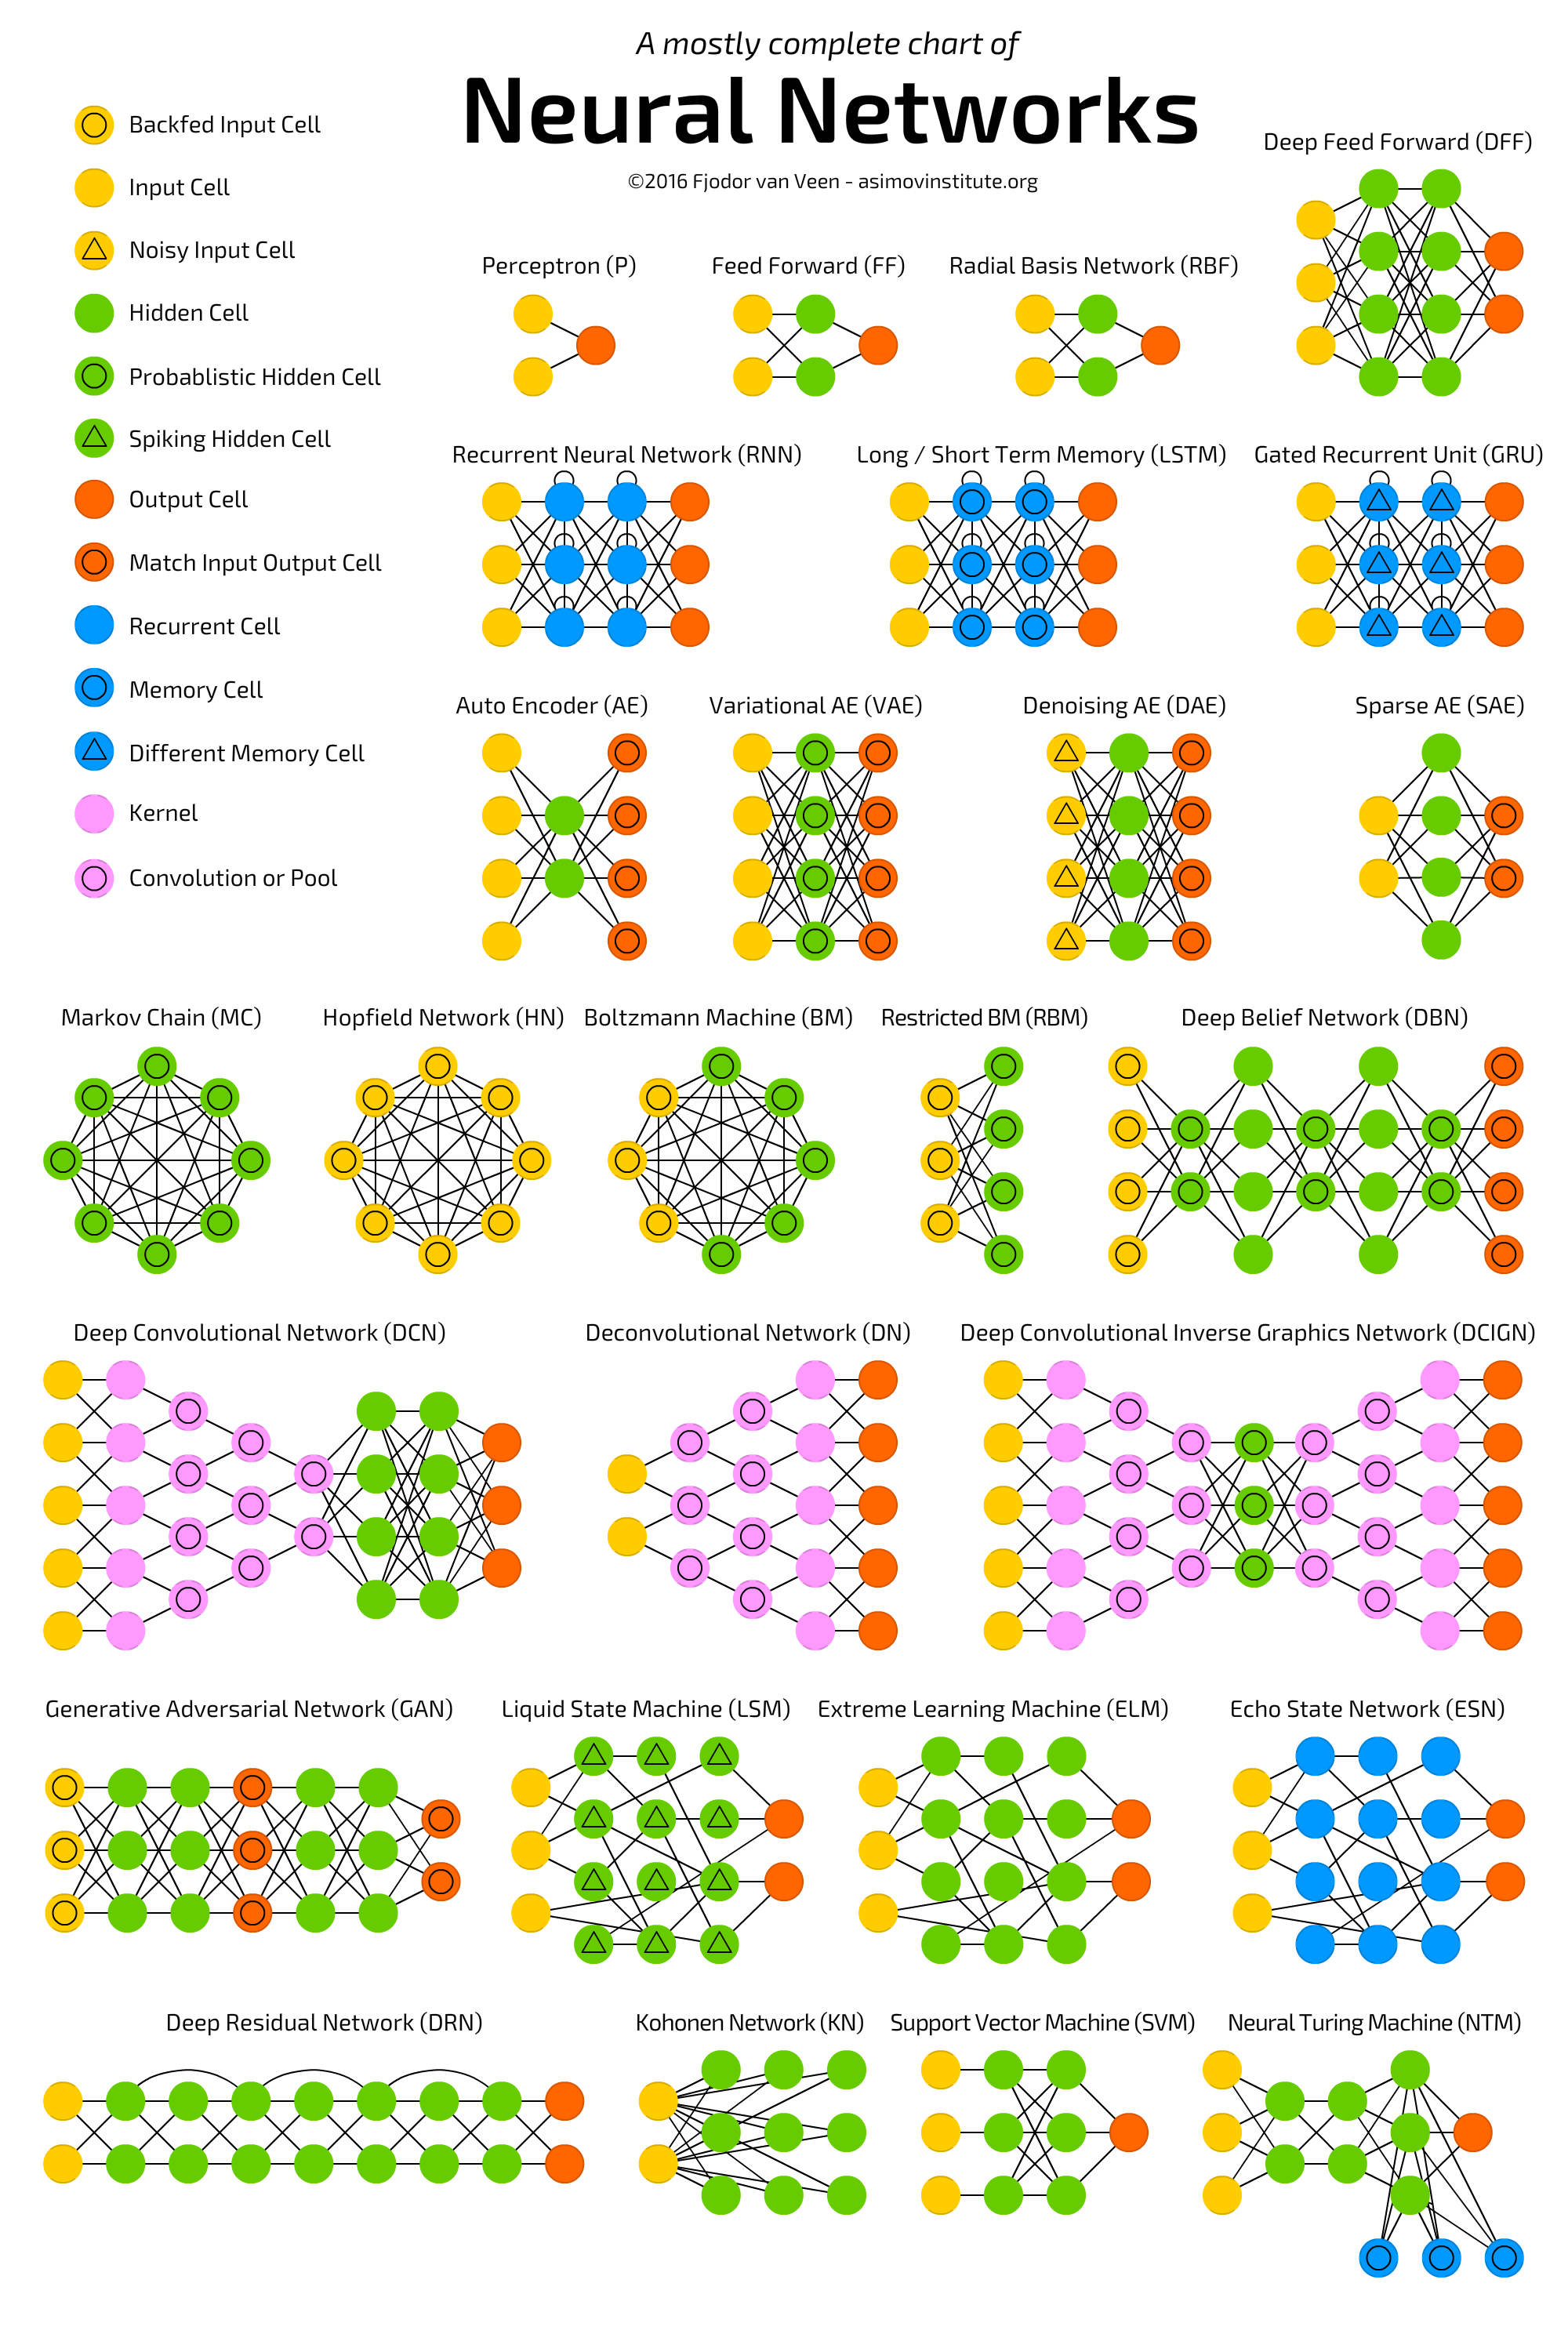
\includegraphics[width=\textwidth]{nnzoo}
  \caption{El zoológico de redes neuronales conocido hasta 2016.
    (Tomado de \url{http://www.asimovinstitute.org}.)
    \cite{website:theasimovinstitute}
  }
\end{figure}

De lo anterior, surge la subrama conocida como \textbf{aprendizaje profundo} y que es la que trae consigo mejoras\
considerables en tareas computacionalmente intratables. Entre los ejemplos que justifican este \emph{boom} tecnológico,\
está el procesamiento de señales de audio, el reconocimiento de rostros, el dominio del juego de mesa chino ``go'',\
la traducción automática de un idioma a otro, la predicción del comportamiento de una bolsa de valores, el reconocimiento\
de imágenes y la generación automática de descripciones de imágenes. Las dos tareas mencionadas al final son la\
\emph{raison d'être} de esta tesis.

\section{Objetivo y metas de la tesis}

\noindent
El presente trabajo busca explorar algunas de las técnicas más relevantes de la actualidad en inteligencia\
artificial. Para ello, se diseñará e implementar un sistema computacional que sea capaz de extraer las características más importantes\
que relacionan una imagen con su leyenda en un meme, utilizando herramientas de aprendizaje profundo. A partir\
de lo anterior, dada una imagen desconocida por el sistema, producir la leyenda que más haga sentido para formar\
un meme, con los conceptos (características) aprendidos en el primer paso.\par
En la consecución de lo anterior, se habrá de lograr las siguientes metas:
\begin{itemize}
\item Recolectar una importante cantidad de memes de internet, clasificándolos por idioma.\
  La mayor parte de dicho conjunto de datos será para entrenar a la red neuronal que se desarrollará,\
  ¿mientras que la otra será para evaluar el desempeño de la misma?.
\item Extraer la leyenda (texto) de cada imagen, de manera que ambas partes queden separadas\
  pero sin perder su asociación.
\item Diseñar e implementar la red neuronal profunda que extraerá las principales características de cada imagen\
  y su leyenda asociada.
\item Implementar un mecanismo para digitalizar las imágenes y que la red neuronal sea capaz de trabajar\
  con éstas y sus leyendas asociadas.
\item Entrenar la red neuronal con el conjunto de datos recolectado de Internet.
\item Evaluar el desempeño de la salida de la red, asociando imagen con leyenda. \st{Hacer cuantas iteraciones}\
  \st{sean necesarias para mejorar la calidad de los memes producidos por la misma}.
\end{itemize}

\section{Estructura de la tesis}

\begin{enumerate}
\item Introducción
\item Trabajo relacionado
\item Aprendizaje profundo
\item Red neuronal para descripciones de memes
\item Evaluación del desempeño de la red
\item Conclusiones
\end{enumerate}
